%% ****** Start of file aiptemplate.tex ****** %
%%
%%   This file is part of the files in the distribution of AIP substyles for REVTeX4.
%%   Version 4.1 of 9 October 2009.
%%
%
% This is a template for producing documents for use with 
% the REVTEX 4.1 document class and the AIP substyles.
% 
% Copy this file to another name and then work on that file.
% That way, you always have this original template file to use.

%\documentclass[aip,jap,numerical,preprint]{revtex4-1}
\documentclass[twocolumn,secnumarabic,amssymb, nobibnotes, aps, pra]{revtex4}
\newcommand{\revtex}{REV\TeX\ }
\newcommand{\classoption}[1]{\texttt{#1}}
\newcommand{\macro}[1]{\texttt{\textbackslash#1}}
\newcommand{\m}[1]{\macro{#1}}
\newcommand{\env}[1]{\texttt{#1}}
\setlength{\textheight}{9.5in}

\usepackage{amsmath}
\usepackage{graphicx}
\usepackage{booktabs}
\usepackage{color}
\usepackage{enumerate}

%\draft % marks overfull lines with a black rule on the right

\begin{document}

%Title of paper
\title{Absorbtion of Beta and Gamma Radiation
% \large{Methods of experimental physics} \\ 
 %\normalsize{PHYS 413}
 }

% repeat the \author .. \affiliation  etc. as needed
% \email, \thanks, \homepage, \altaffiliation all apply to the current
% author. Explanatory text should go in the []'s, actual e-mail
% address or url should go in the {}'s for \email and \homepage.
% Please use the appropriate macro foreach each type of information

% \affiliation command applies to all authors since the last
% \affiliation command. The \affiliation command should follow the
% other information
% \affiliation can be followed by \email, \homepage, \thanks as well.
\author{Jason Morgan}
\affiliation{Department of Physics, Old Dominion University, Norfolk VA 23529}
\date{\today}


\begin{abstract}

The purpose of this lab is to study the behaviour of beta and gamma rays as they pass through aluminum and lead respectivly. We will measue the value of $\mu$ for weak gamma radiation and the end point energy of beta particles emitted from Strontium$^{90}$.

\end{abstract}

\maketitle
\section{Introduction}

Beta and gamma rays exhibit different behaviour when passing through a medium.  Beta rays are electrons ejected from the nuculeus is an atom when a proton decays to a nutron.  Beta rays display a linear loss of energy as they pass through a material.  Gamma rays display an exponential decay and are never truely stopped by a material used for attenuation.  Gamma rays adhere the equation below when passing through a material.

\begin{equation}
I = I_0 e^{-\mu * x}
\label{Attenuation of gamma rays}   %label the equation
\end{equation}
where x is the thickness of the material, $I_0$  is the initial intensity of radiation and $\mu$ coefficient of attenuation of the material the radiation is passing through. 

Beta particles adhere to a much more complex formula for intensity after passing through a certain amount of material.  Instead we will use an approximate formula that relates the energy of the electron to the range in a given material

\begin{equation}
r = \frac{0.412 \frac{g}{cm^2}}{\rho} (E)^{1.29}
\label{eq:beta}   %label the equation
\end{equation}
where r is in cm, E is in MeV, and  $\rho$ is the density of the attenuating material in $\frac{g}{cm^3}$


\section{Experimental setup and procedures}


\begin{figure}[h]
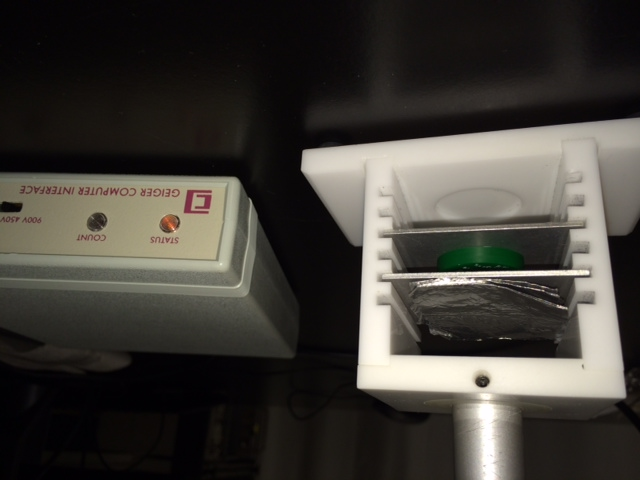
\includegraphics[scale=0.4,angle=180]{Setup.jpg}% Here is how to import EPS art
\caption{Experimental set for attenuation of beta and gamma rays.  The images shows the stand holding the attenuating material (aluminum foil), the radioactive source (Strontium 90) and the geiger counter. }
\label{fig:setup}
\end{figure}

\begin{table} [h]  % Capital letters stronger suggestion
\caption{Geiger Counter Calibration}      %title of the table     
\centering              % centering table
\begin{tabular}{crr} % creating four columns (c stands for ceneter, r for right, l for left)
\hline\hline %inserting double-line
  No & Voltage (V)  & Total Counts   \\
\hline % inserts single-line
1 & 0 & 0   \\
2 & 50 & 0   \\
3 & 100 & 0  \\
4 & 150 & 0  \\
5 & 200 & 0  \\
6 & 250 & 0  \\
7 & 300 & 0  \\
8 & 350 & 152  \\
9 & 400 & 168  \\
10 & 450 & 167 \\

\hline % inserts single-line
\end{tabular}
\label{tab:tuning}
\end{table}

The data used for calibration of the geiger counter are shown in table \ref{tab:tuning}. The readings plateaued between 400V and 500V and we set the geiger counter to 425V for the duration of data collection.


\section{Results and Discussion}



\subsection{Results for Attenuation of Beta Rays}

The graph in Fig \ref{fig:beta} shows the intensity of beta particles as a function of the thickness of aluminum between the source and the detector.  It drops below background at 0.317 $\pm$ 0.03 cm.  The error is calculated from the average of the individual errors in each measurement.  This yields a value of 1.78 $\pm$ 0.4 MeV using Eq \ref{eq:beta} for this value of r.  This is within the ranges of energies emitted by Strontium$^{90}$.  Strontium$^{90}$ undergoes two decays.  One with an energy of 0.547 MeV and one with an energy of 2.38 MeV.  The energy measured should be that of the most energetic beta emission of 2.38 MeV.  This gives a percentage error of 25%

The error in our measurement of thickness is much larger than it should be.  This is due to the method we choose to calculate the thickness.  The aluminum plates were measured with a micrometer which introduced an expected amount of error due to it's accuracy.  The foil was taked form the standard thicknes of heavy duty aluminum foil.  This resulted in an error of $\pm$ 0.005 for each sheet.  This error must be multiplied by the number of sheets for each trial which means it is less and less accurate as the number of sheets is increased.  

To reduce these errors, the entire thickness of all the sheets should have been measured to reduce this error.  Additionally, more trials at different thickness should have been taken.  This would allow the point at which the intensity dropped to background to be identified more accurately.


\subsection{Results for Attenuation of Gamma Rays}

The graph in Fig \ref{fig:gamma} shows the intensity of gamma rays as a function of the thickness of Lead between the source and the dector.  The graph does not include the data point for no attenuating material.  Due to errors in our procedure this value was not taken correctly and has been thrown out.  The data point was supposed to be taken with the alumninum plate in place and this measurement did not include the plate.  The absence of the aluminum plate would allow beta particles that are a product of the decay process to make it to the detector.  These particles are completely blocked by the first sheet of lead causing the reading to be higher without the aluminum plate.

The value of $\mu$ is found by fitting the data with an exponential function resulting in a value for $\mu$ of 2.20 $\pm$ 0.1 cm$^{-1}$.  The values of $\mu$ are given in the form $\frac{\mu}{\rho}$ which yields  0.19 $\pm$ 0.001 $cm^{2}/g$ for the 0.662 MeV gamma radiation.  The expected value is between 0.11 and 0.12 $cm^{2}/g$ based on sources [1] [2].  This gives a percentage error of 65%.  

This error is very large.  Initially it was thought that gamma ray scatering could have been the result of much of this error.  This would have resulted in a lower value of $\mu$ than expected since it would result in more gamma rays reaching the detector.  Threfore it cannot be the primary source of the error.  To fully determine the cause of the error involved in the results the experiment would need to be performed again taking care to eliminate as many sources of error as possible.  More data points should be taken when doing so to further reduce the errors.  


\section{Conclusion}

This lab was a good introduction to data gathering and analysis. The numbers did not match the expected values very well but analysing the errors involved in the measurements was a good learning experience. 


\begin{figure}[b]
\begin{center}
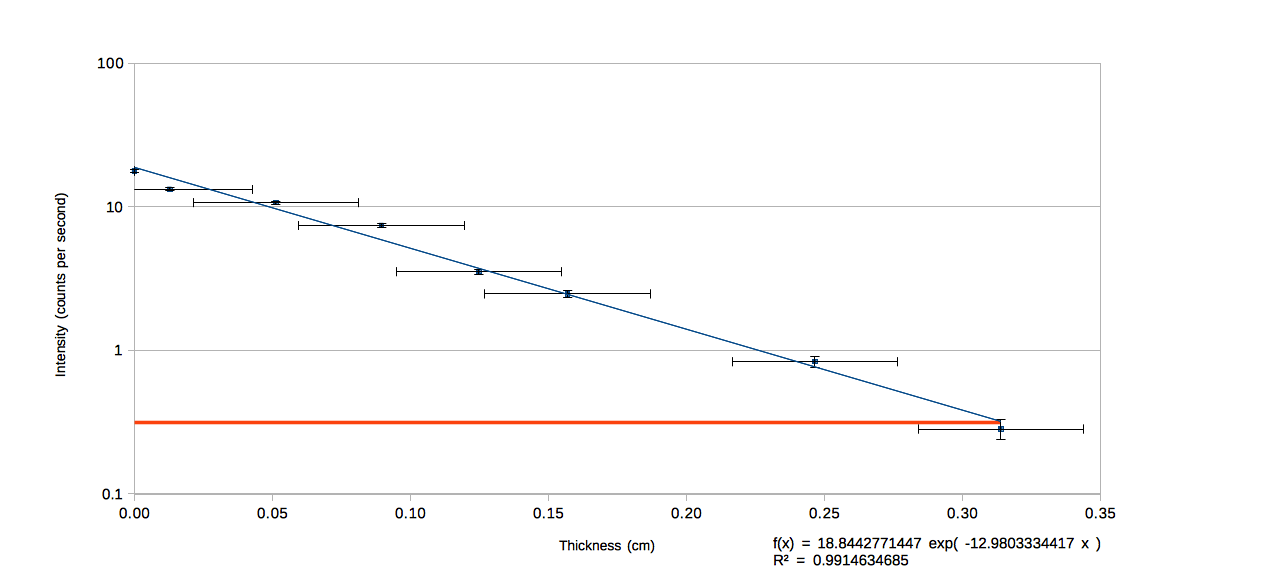
\includegraphics[scale=0.7]{BetaDataAnalysis.png}
\end{center}
\caption{Attenuation of beta particles by aluminum, y error bars may be too small to discern.}
\label{fig:beta}
\end{figure}

\begin{figure}[b]
\begin{center}
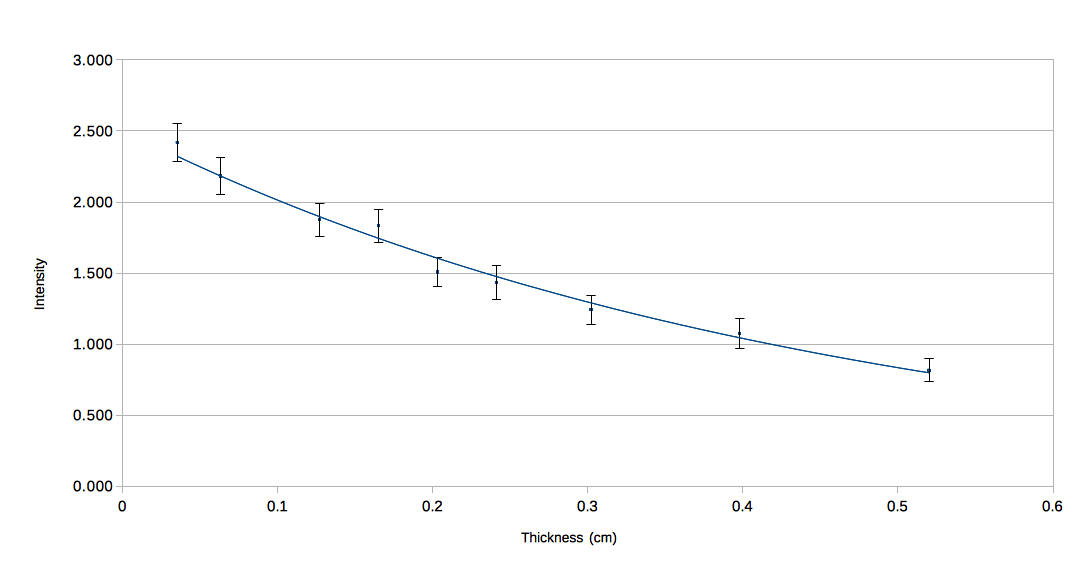
\includegraphics[scale=.7]{GammaDataAnalysis.png}
\end{center}
\caption{Attenuation of gamma rays by lead.  $I = (2.5 \pm 0.1)e^{-(13.0 \pm 0.1) }$ $R^2 = 0.99$}
\label{fig:gamma}
\end{figure}

%Write down references
%-----------------------------------
\begin{thebibliography}{5}
\bibitem{mcalister1} Daniel R. McAlister, \textit{Gamma Ray Attenuation Properties of Common Shielding Materials}, (PG Research Foundation, 1955 University Lane Lisle IL, 2013).
\bibitem{darbas1} Andrius Poškus, \textit{ATTENUATION OF GAMMA RAYS}, (Vilnius University Faculty of Physics, Laboratory of Atomic and Nuclear Physics, 2012).
\bibitem{csmahajan1} C S Mahajan, \textit{Mass attenuation coefficients of beta particles in elements}, (Bezonji Science college, Jalna India, 2012).
\end{thebibliography}


\end{document}
%
% ****** End of file aiptemplate.tex ******
